\section{Results}

\subsection{Context improves requested-interval recognition}
\begin{table}[tb]
\centering\small
\caption{Requested-interval WER (\%). Each arm uses its development-selected decoder. Targets are at most two seconds with up to 0.64 s of context per side. Source clusters are recording identifiers, not verified speakers.}
\label{tab:primary}
\begin{tabular}{lrrrrr}
\toprule
Corpus & Clips & Sources & Crop A & Direct B & Projection C \\
\midrule
VLR & 11,306 & 61 & 58.602 & 50.579 & 50.434 \\
LRS2 & 1,243 & 354 & 24.099 & 23.609 & 21.733 \\
Spanish & 934 & 12 & 85.451 & 81.527 & 80.170 \\
ViCocktail & 1,167 & 20 & 51.767 & 49.179 & 48.193 \\
\bottomrule
\end{tabular}
\end{table}

\begin{table}[tb]
\centering\small
\setlength{\tabcolsep}{4pt}
\caption{Matched-decoder requested-interval WER (\%). Negative C--B favors projection. Brackets give explanatory pointwise 95\% paired-source bootstrap intervals from 10,000 draws; the primary adjusted family is reported separately.}
\label{tab:matched}
\begin{tabular}{llrrrl}
\toprule
Corpus & Decoder & A & B & C & C--B [95\% CI] (pp) \\
\midrule
VLR & Greedy & 58.602 & 50.579 & 50.434 & -0.145 [-0.181, -0.110] \\
VLR & Pure CTC & 58.971 & 50.862 & 50.691 & -0.172 [-0.214, -0.129] \\
LRS2 & Greedy & 30.527 & 28.749 & 28.471 & -0.277 [-0.463, -0.126] \\
LRS2 & Pure CTC & 30.250 & 28.536 & 28.226 & -0.310 [-0.500, -0.155] \\
Spanish & Greedy & 83.181 & 81.824 & 80.870 & -0.954 [-1.390, -0.672] \\
Spanish & Pure CTC & 83.203 & 81.718 & 80.764 & -0.954 [-1.429, -0.670] \\
ViCocktail & Greedy & 55.540 & 52.643 & 52.524 & -0.119 [-0.213, -0.011] \\
ViCocktail & Pure CTC & 55.520 & 52.623 & 52.464 & -0.159 [-0.249, -0.061] \\
\bottomrule
\end{tabular}
\end{table}

Projection improves over crop-first recognition in all four principal
comparisons (Table~\ref{tab:primary}). The reduction ranges from
\PrimaryGainMin{} to \PrimaryGainMax{} percentage points, and all four
family-adjusted intervals favor projection. The result concerns the same
requested target within each corpus: it is not a comparison between a short
target transcript and a longer full-clip transcript.

Contextual direct decoding captures much of the benefit. For VLR, moving from
crop-first to contextual direct changes WER from 58.602\% to 50.579\%;
projection provides a further 0.145-point reduction. The additional
selected-system reductions are 1.876 points on LRS2, 1.357 on Spanish, and
0.986 on ViCocktail. The adjusted Spanish C--B interval includes zero;
the other three adjusted intervals favor C.

Matched decoders give a more specific interpretation
(Table~\ref{tab:matched}). Under pure CTC, the C--B improvements are
0.172, 0.310, 0.954, and 0.159 points, with explanatory paired-source 95\%
intervals favoring C in all four settings. Thus projection contributes beyond
contextual state cropping at the principal operating point, while contextual
encoding accounts for the larger improvement. The selected-system comparisons
add the effect of each arm's development-selected decoder. Spanish illustrates
the relevance of both views: crop-first greedy and pure CTC outperform its
selected hybrid on assessment.

\paragraph{Decoder sensitivity.}
Projection does not outperform contextual direct at every decoder setting.
On the separate VLR development screen, pure CTC with zero blank bias gives
60.085\% for C versus 59.659\% for B: a C--B difference of +0.426 points
with pointwise 95\% interval [+0.105, +0.802]. VLR greedy decoding also
favors B by point estimate at all three tested blank biases.
On ViCocktail, a hybrid length bonus of +1 gives 45.302\% for C versus
44.214\% for B (+1.088 points, interval [-0.340, +2.739]); this comparison
retains the respective CTC weights of 0.1 and 0.5. These development results
show that the readout ranking depends on decoder configuration. They do not
retune or replace the frozen assessment results (Appendix~\ref{app:decoder-sensitivity}).

\subsection{Actual context availability explains aggregate readout effects}
\label{sec:availability}
\begin{figure}[tb]
 \centering
 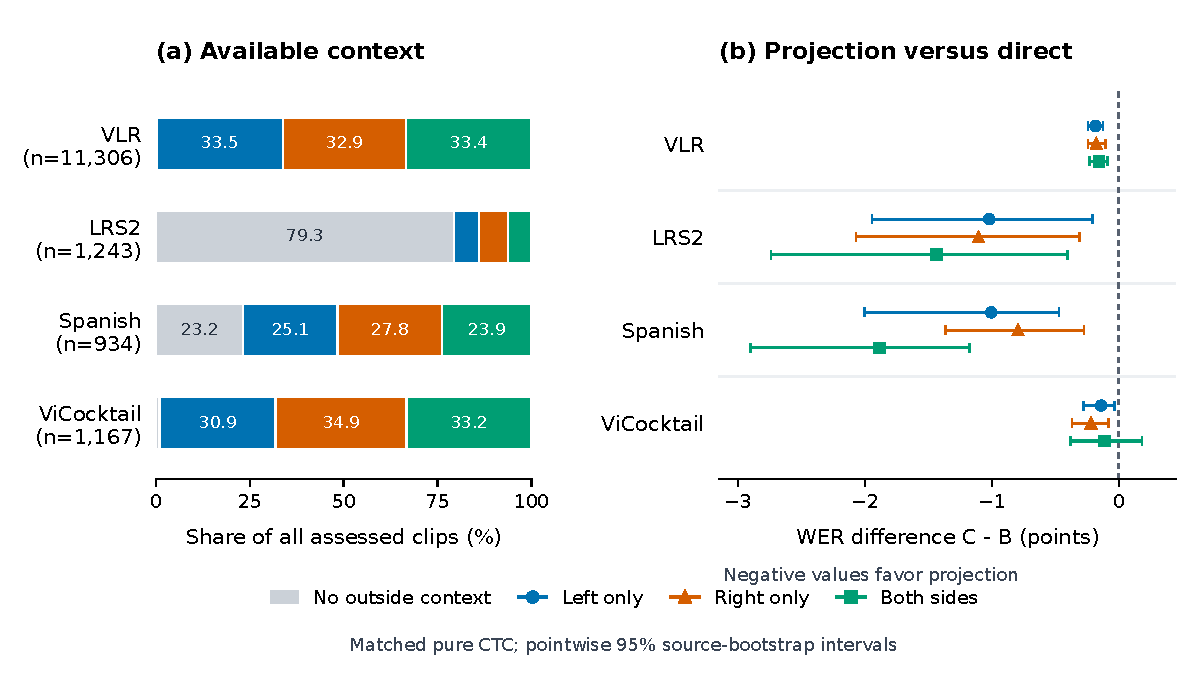
\includegraphics[width=\linewidth]{fig_Context_Availability.pdf}
 \caption{Post-hoc analysis of the frozen principal assessment, using the
 same pure-CTC decoder for A/B/C. (a) All clips partitioned by actual context
 outside the target. (b) C--B WER differences within the three groups with
 outside context; negative values favor projection. Bars are pointwise 95\%
 paired-source bootstrap intervals, without multiplicity adjustment. No-context
 predictions are identical across A/B/C. Groups differ in request position and
 clip duration, so their differences do not isolate causal left/right effects.
 Full counts and WERs appear in Table~\ref{tab:context-availability}.}
 \label{fig:context-availability}
\end{figure}
A post-hoc stratification separates requests by actual outside context
(Figure~\ref{fig:context-availability}; Table~\ref{tab:context-availability}).
With matched decoders, A/B/C predictions are identical when the request covers
the available video. This occurs on
986 of 1,243 LRS2 clips (79.3\%), compared with 27/11,306 VLR, 217/934 Spanish,
and 11/1,167 ViCocktail clips. The LRS2 aggregate thus mixes many identity
cases with requests that permit contextual readout.

For the LRS2 groups with left, right, and both-sided context (83, 96, and
78 clips), the pure-CTC C--B reductions are 1.020, 1.106, and 1.434 points;
each corresponding pointwise interval favors C. The reductions across these
three groups range from 0.158 to 0.183 points on VLR and from 0.794 to
1.883 on Spanish. ViCocktail has smaller reductions of 0.115--0.220 points,
and its both-context interval includes zero. The complete principal endpoint
retains all clips, including those without outside context. This explanatory
analysis uses pointwise 95\% intervals on previously evaluated data; it is
not an independent confirmation or a change to the primary comparison family.
Directional effects of context are tested separately by the interventions below.

\subsection{Visual alignment contributes to output selection}
\begin{table}[tb]
\centering\small
\caption{Development-selected requested-interval WER (\%). The uniform controls allocate the same decoded sequence as C. Full-clip lookup processes unrestricted input and returns the same requested target; it is a different input-budget baseline.}
\label{tab:allocation}
\begin{tabular}{lrrrr}
\toprule
Corpus & Aligned C & Uniform words & Uniform tokens & Full-clip lookup \\
\midrule
VLR & 50.434 & 56.168 & 56.066 & 42.720 \\
LRS2 & 21.733 & 22.842 & 23.071 & 21.553 \\
Spanish & 80.170 & 82.821 & 82.694 & 78.770 \\
ViCocktail & 48.193 & 52.125 & 52.364 & 45.495 \\
\bottomrule
\end{tabular}
\end{table}

Table~\ref{tab:allocation} compares allocation rules applied to the same
contextual prediction. Aligned projection has lower error than both uniform
rules in each principal setting. This comparison cannot be explained by a
different generated transcript: the alternatives share predicted tokens and
differ only in their assignment to the requested interval.

Unrestricted full-clip lookup has the lowest target error in these settings.
It provides the accuracy reference when the application can process the entire
video. The bounded alternatives answer the same request using a prescribed
observation interval, exposing the accuracy cost of that input constraint.

\subsection{Real context supplies more than additional frames}
\begin{table}[tb]
\centering\small
\caption{Real context versus repeated-boundary padding, restricted to clips with available outside context. Both conditions preserve target pixels and input length. Intervals are explanatory pointwise 95\% source-bootstrap intervals.}
\label{tab:intervention}
\begin{tabular}{llrl}
\toprule
Corpus & Decoder regime & Clips & Real--repeat difference (pp) \\
\midrule
VLR & Selected & 254 & -4.219 [-5.905, -2.605] \\
VLR & Pure CTC & 254 & -4.430 [-6.026, -2.913] \\
LRS2 & Selected & 48 & -7.767 [-14.286, -2.222] \\
LRS2 & Pure CTC & 48 & -7.443 [-12.333, -2.857] \\
Spanish & Selected & 202 & -9.635 [-11.979, -7.156] \\
Spanish & Pure CTC & 202 & -3.043 [-4.700, -1.230] \\
ViCocktail & Selected & 254 & -9.286 [-11.456, -7.326] \\
ViCocktail & Pure CTC & 254 & -6.066 [-8.193, -4.103] \\
\bottomrule
\end{tabular}
\end{table}

On clips with outside context, real video improves over repeated-boundary
padding under both selected systems and matched pure CTC
(Table~\ref{tab:intervention}). The target pixels and input length are
unchanged in this contrast. Thus the benefit is not explained solely by a
longer tensor or a different target crop.
The complete intervention table in Appendix~\ref{app:context-controls}
also compares single-sided and reversed context. Both real margins outperform
either margin alone in those settings, while the preferred individual side
varies across corpus/model conditions.

These interventions establish the value of real neighboring content over the
tested alternatives. They affect motion continuity together with speech
information, so the contrast concerns visual context as a whole.

\subsection{Duration changes the opportunity to use context}
\begin{figure}[tb]
 \centering
 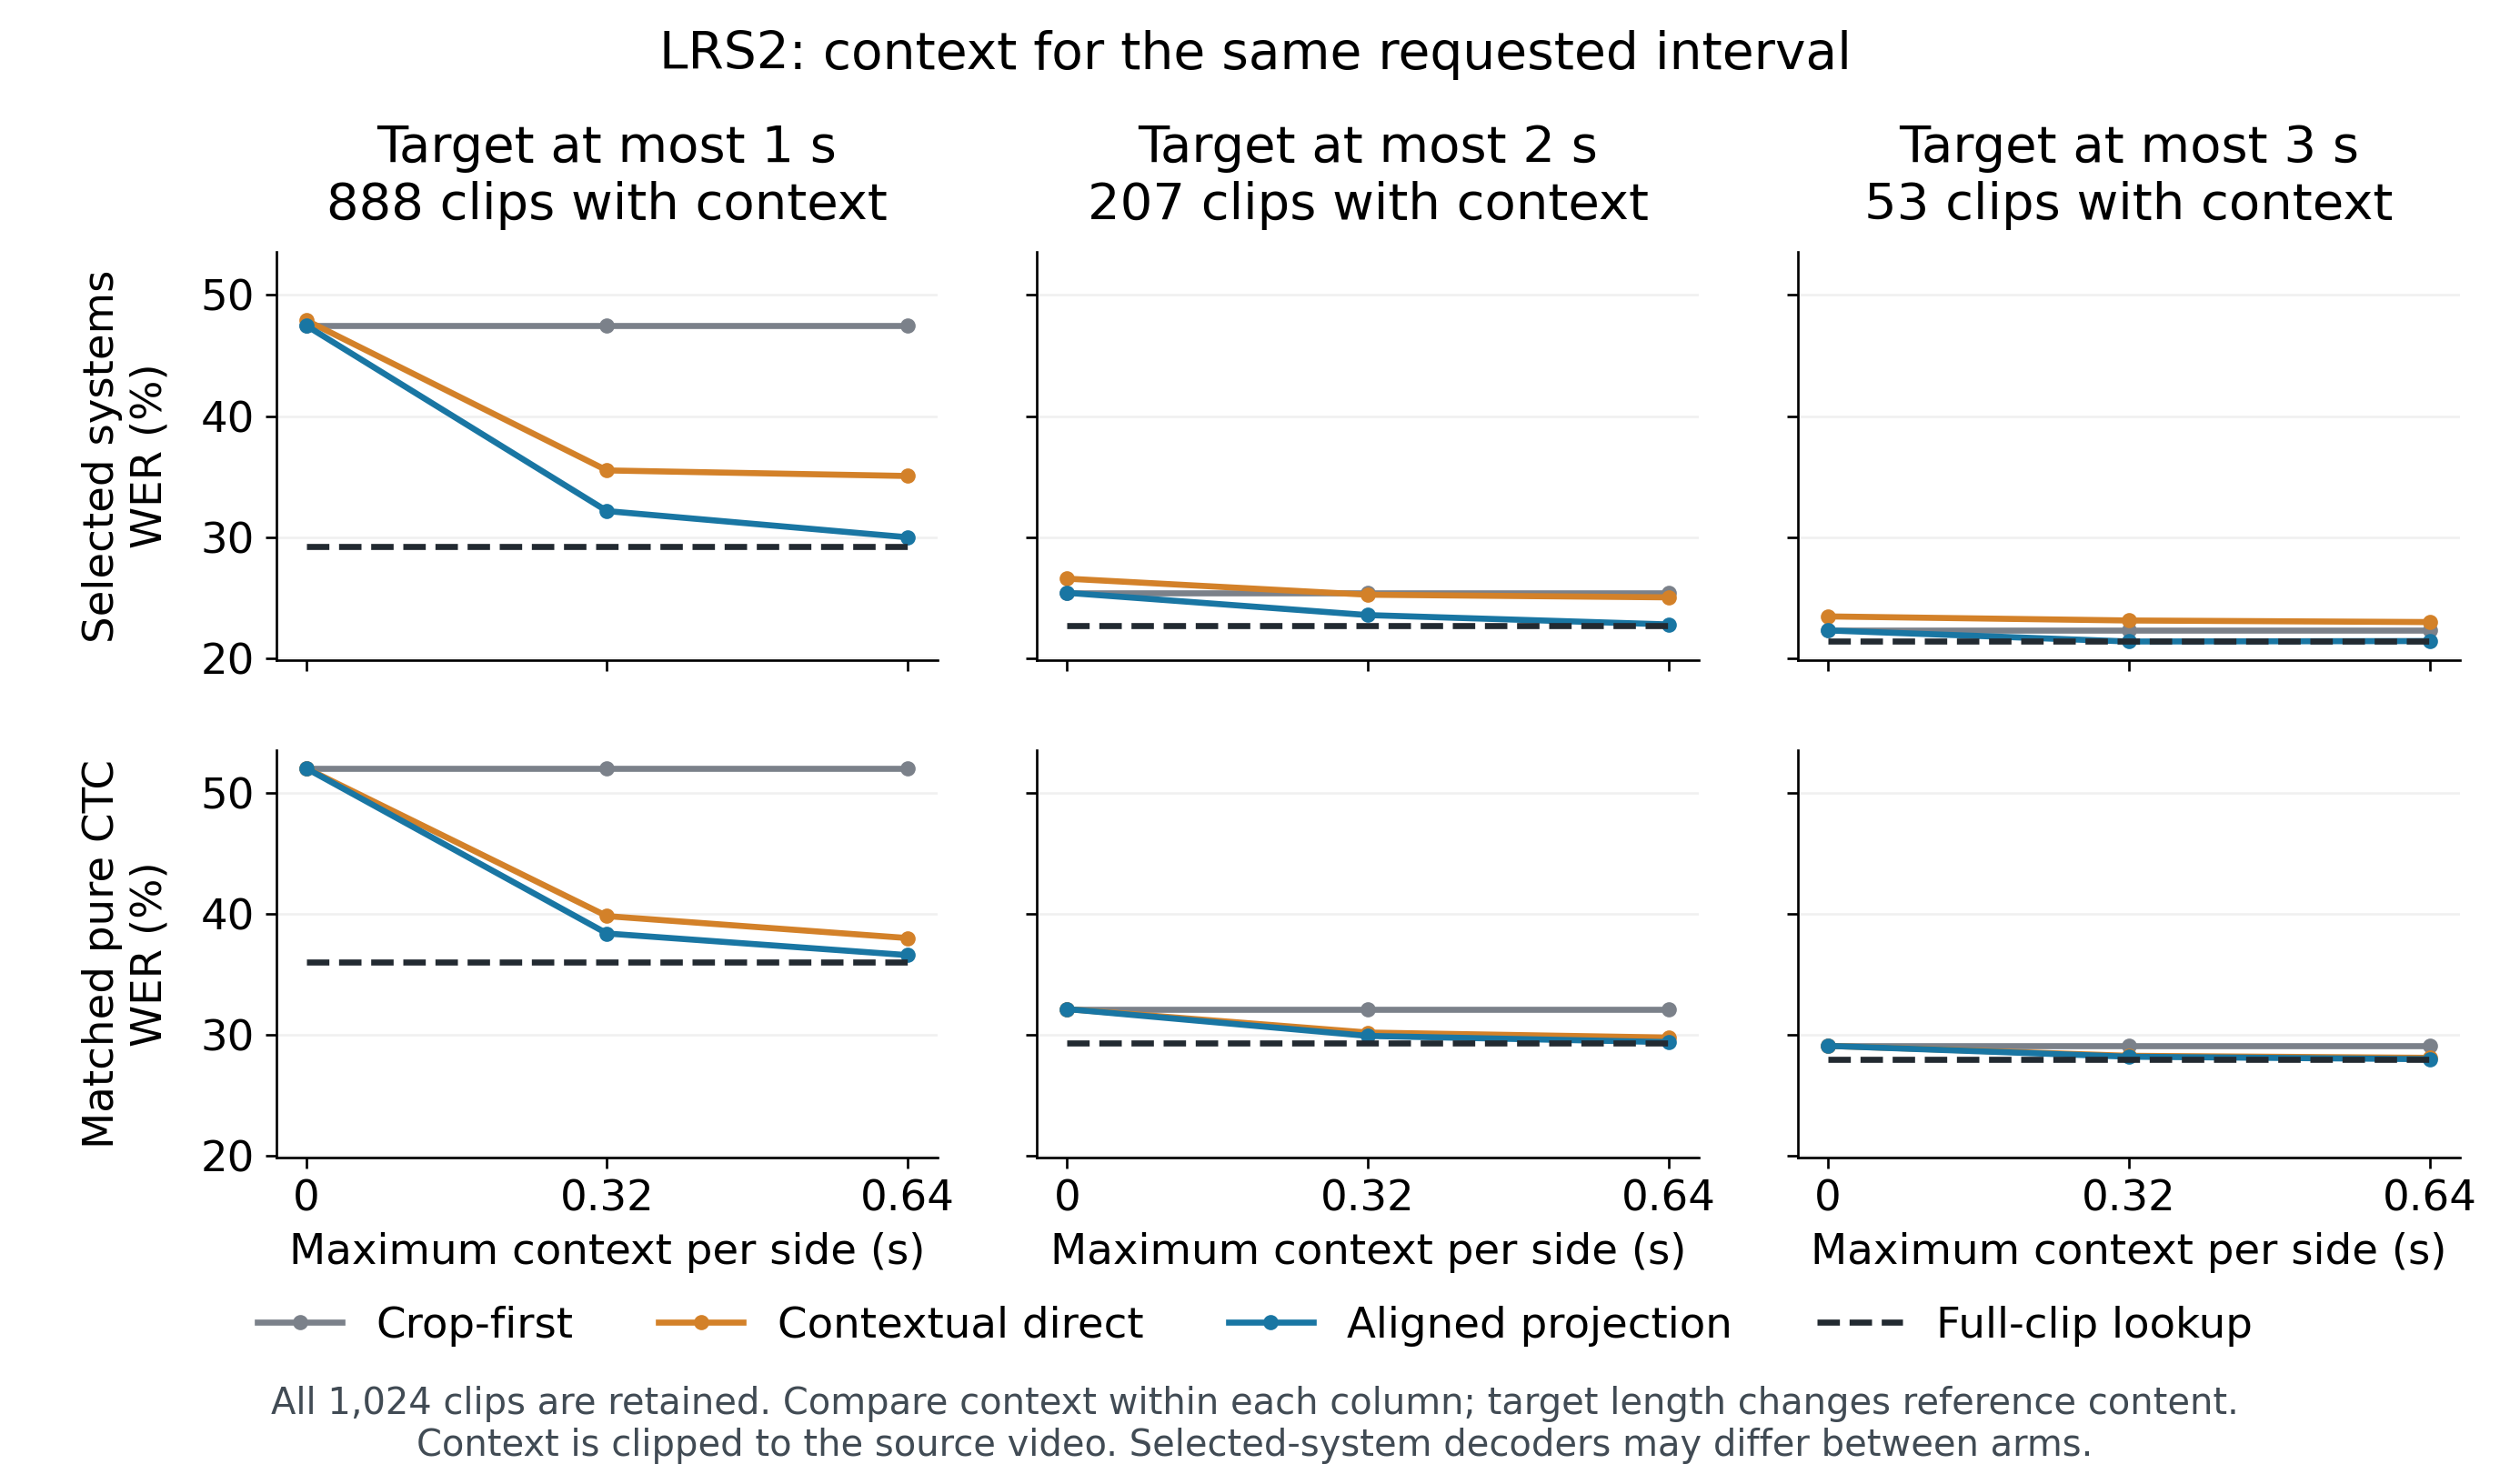
\includegraphics[width=\linewidth]{fig_EN_B1_Context_Grid.png}
 \caption{LRS2 duration experiment on 1,024 clips. Compare context budgets
 within a column: the target text is fixed there. Columns change the requested
 content and are not competing estimates of the same transcript. Both
 development-selected systems and matched pure CTC are shown.}
 \label{fig:english-context}
\end{figure}
The one-second LRS2 target provides a substantial context opportunity
(Figure~\ref{fig:english-context}). Selected projection decreases from
\EnglishOneNoContext{}\% without context to 32.151\% at a 0.32-second
per-side allowance and \EnglishOneContext{}\% at 0.64 seconds. At the latter
budget, contextual direct is 35.049\%. Under matched pure CTC, direct and
projection are 37.974\% and 36.566\%, a 1.408-point reduction with pointwise
source-bootstrap interval [1.023, 1.819] when expressed as an improvement.

The opportunity shrinks as the target covers more of these short clips.
Outside context exists for 888 of 1,024 clips at a one-second target,
207 at two seconds, and only 53 at three seconds. With a one-second target
and a nominal 0.64-second per-side budget, mean actual input is 1.526 seconds;
mean total added context is 0.541 seconds.

The complete VLR grid provides a different duration distribution
(Appendix~\ref{app:duration}). Outside context exists for 1,022 clips at
one- and two-second targets, and 1,012 at three seconds. With greedy decoding,
one-second crop-first WER is 82.659\%, contextual direct with the larger
budget is 57.018\%, and projection is 56.490\%. Its 0.529-point advantage
over direct has pointwise interval [0.222, 0.847] when expressed as a reduction.
Pure CTC gives a corresponding 0.608-point reduction [0.230, 0.996].
At two- and three-second targets, the incremental greedy C--B differences
are -0.053 and -0.044 points, with intervals including zero. Duration therefore
affects both the availability of outside evidence and the benefit of retaining
context through decoding. Context budgets are compared within a fixed target;
different target lengths request different text.

The Spanish and ViCocktail grids extend this comparison to different
corpus/model conditions (Appendix~\ref{app:duration}). At the 0.64-second
allowance, selected Spanish projection changes from 105.737\% to 87.330\%
for the one-second target, and from 89.499\% to 79.991\% for two seconds.
Under matched pure CTC, its improvements over contextual direct are
2.270, 1.558, and 0.830 points for one-, two-, and three-second targets;
the corresponding pointwise intervals all favor projection.
ViCocktail shows a different readout profile. Selected projection improves
from 70.109\% to 59.447\% for one-second requests, but the matched pure-CTC
C--B difference is +0.067 points with interval [-0.153, +0.308]. At two and
three seconds, the matched reductions are 0.133 and 0.102 points. A sizable
context gain can therefore coexist with little additional projection gain.

Increasing context beyond 0.32 seconds also has a corpus-dependent return.
On one-second targets with outside context, the matched-CTC change from
0.32 to 0.64 seconds per side is -3.574 points on VLR, -2.064 on LRS2,
-0.585 on Spanish, and -2.345 on ViCocktail. The Spanish interval includes
zero, whereas the other three favor the larger budget. These paired results
support evaluating context budgets for the intended request and recognizer;
they do not establish an adaptive policy or a universal optimal budget.

\subsection{Whole-transcript recognition favors full input}
\begin{table}[tb]
\centering\small
\caption{Whole-transcript WER (\%) under matched pure CTC, 512 clips per corpus. The shared sliding schedule partitions each clip into balanced targets of at most two seconds with 0.64 s context per side. Full-clip output uses the same reference transcript. Intervals are pointwise source-bootstrap intervals.}
\label{tab:whole}
\resizebox{\textwidth}{!}{%
\begin{tabular}{lrrrl}
\toprule
Corpus & Direct sliding & Projected sliding & Full clip & C--F (pp) \\
\midrule
VLR & 48.667 & 48.452 & 42.877 & +5.575 [+4.641, +6.491] \\
LRS2 & 28.936 & 28.186 & 27.286 & +0.900 [+0.158, +1.631] \\
Spanish & 78.866 & 77.353 & 74.558 & +2.795 [+1.622, +4.239] \\
ViCocktail & 47.723 & 47.691 & 43.756 & +3.935 [+3.066, +4.743] \\
\bottomrule
\end{tabular}%
}
\end{table}

Projected sliding can improve direct sliding, but full-clip recognition
remains stronger on the same complete transcripts
(Table~\ref{tab:whole}). Joining contextual target CTC scores and decoding
once removes some concatenation errors without closing that gap.
At the two-second schedule, this control removes 25, 0, 2, and 10 errors
relative to projected pure-CTC sliding on VLR, LRS2, Spanish, and ViCocktail.

The error balance varies across corpora. Under matched CTC, projected sliding
relative to full-clip decoding
adds 431 substitutions and 589 insertions on VLR while reducing deletions
by 451; Spanish instead adds 220 deletions and 20 substitutions while reducing
insertions by 33. These different error balances are compatible with disruption
of recognition and repeated local decisions, extending beyond duplicated text
at window seams.

\subsection{Query workload determines the cost advantage}
\begin{table}[tb]
\centering\small
\caption{Matched pure-CTC response cost on 32 stratified calibration clips per corpus. Values are across-clip medians after reducing three fresh sessions to one median per clip. All arms use beam 40 with token pruning 64 on the same GTX 1650 Ti. The final column counts paired clips on which C is faster than F. Short clips can deduplicate requests; these descriptive timings do not measure assessment accuracy.}
\label{tab:matched-query-cost}
\begin{tabular}{lrrrrrr}
\toprule
Corpus & Queries & A (s) & B (s) & C (s) & F (s) & C $<$ F \\
\midrule
VLR & 1 & 0.390 & 0.432 & 0.623 & 1.221 & 28/32 \\
VLR & 3 & 1.159 & 1.269 & 1.658 & 1.034 & 2/32 \\
VLR & 5 & 1.954 & 2.128 & 2.865 & 1.093 & 0/32 \\
LRS2 & 1 & 0.338 & 0.362 & 0.441 & 0.455 & 22/32 \\
LRS2 & 3 & 1.026 & 0.979 & 0.459 & 0.431 & 6/32 \\
LRS2 & 5 & 1.681 & 1.599 & 0.561 & 0.462 & 6/32 \\
Spanish & 1 & 0.378 & 0.419 & 0.589 & 0.987 & 29/32 \\
Spanish & 3 & 1.149 & 1.227 & 1.584 & 0.989 & 9/32 \\
Spanish & 5 & 1.903 & 2.037 & 2.785 & 1.014 & 0/32 \\
ViCocktail & 1 & 0.350 & 0.383 & 0.552 & 0.677 & 28/32 \\
ViCocktail & 3 & 1.033 & 1.132 & 1.458 & 0.741 & 10/32 \\
ViCocktail & 5 & 1.734 & 1.909 & 2.563 & 0.708 & 5/32 \\
\bottomrule
\end{tabular}
\end{table}

Holding the decoder fixed reveals a consistent workload distinction
(Table~\ref{tab:matched-query-cost}). For one request, projection is faster
than fresh full-clip lookup on 28/32 VLR clips, 22/32 LRS2 clips, 29/32
Spanish clips, and 28/32 ViCocktail clips. Their paired median C--F time
differences are $-0.612$, $-0.027$, $-0.378$, and $-0.083$ seconds.
For five requested intervals, the paired differences become $+1.698$,
$+0.105$, $+1.824$, and $+0.938$ seconds. Full-clip recognition pays its
initial cost once and reuses the resulting transcript and temporal index.
Marginal medians in the table and medians of paired differences describe
different summaries; they need not differ by the same amount.

Projection also has a cost relative to contextual direct decoding. The paired
median C--B difference is positive in all twelve corpus/workload cells,
ranging from 0.017 to 0.754 seconds. Encoding frame counts are identical
between B and C in every paired clip. C generally decodes a longer sequence
and adds alignment, but distinct targets can sometimes share a contextual
prediction. In LRS2, this reuse reduces C's decode count relative to B on
seven clips with three requests and eight with five; C is faster on each of
those clips. This is the cache behavior described in
Section~\ref{sec:query-computation}, not an additional accuracy gain.

The supplement reports selected-system costs, matched tail latency, and memory.
Together with the paired accuracy results, these measurements distinguish the
cost of a bounded request from the benefit of amortizing full-clip recognition
over a session.
